% Provenance (never printed): cycle 3 "La planete Terre" (the shaping of
% landscapes: erosion, transport and deposition by running water; rivers
% from source to mouth; floods); see sources/book1/PROVENANCE.md.
% Book 1, grade 5, chapter 1.
\chapter{Water Shapes the Land}\label{ch:g5:water-shapes-the-land}

All night long, the storm drummed on the roof of the school. In the
morning the sky is clearing, and Lena and Tom run to the little stream
behind the playground. Yesterday it was clear and quiet: they could count
the \omterm{def:g3:stones-pebbles-sand:pebble}{pebbles} on its bed. Today it is wide, fast and brown, the colour of
milky chocolate. It carries twigs, leaves, and something they cannot see
one by one: \omterm{def:g3:stones-pebbles-sand:sand}{mud} and \omterm{def:g3:stones-pebbles-sand:sand}{sand}, torn from its banks and from the fields
upstream.

``Where is all that \omterm{def:g3:stones-pebbles-sand:sand}{mud} going?'' asks Tom. Downstream, a little further
every minute. The stream is carrying the land away, grain by grain. In this
chapter we follow those grains, from the \omterm{def:g3:stones-pebbles-sand:rock}{rock} they come from to the place
where they settle.

\begin{omfigure}
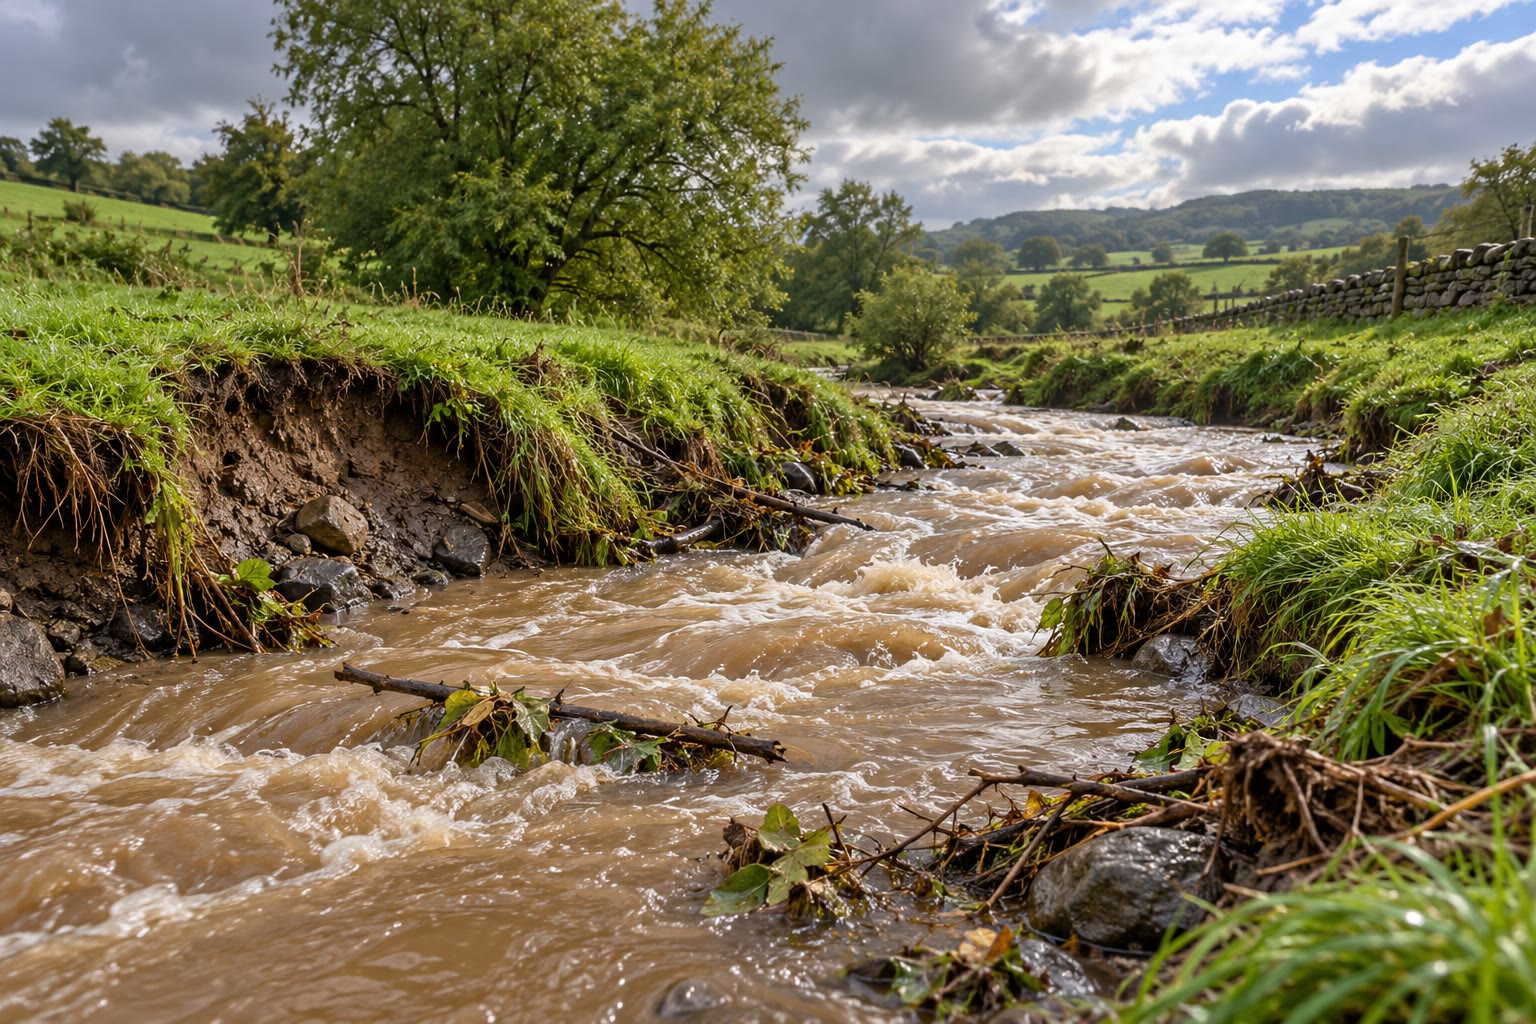
\includegraphics[width=0.5\linewidth]{images/book1/ai/g5-brown-stream.jpg}

{\small A stream the morning after a storm: the water is brown with the \omterm{def:g3:stones-pebbles-sand:sand}{mud}
and \omterm{def:g3:stones-pebbles-sand:sand}{sand} it carries.}
\end{omfigure}

\begin{recall}
\omterm{def:g3:stones-pebbles-sand:rock}{Rock} is the hard material of the Earth; broken into pieces it gives stones,
\omterm{def:g3:stones-pebbles-sand:pebble}{pebbles} rounded by water, \omterm{def:g3:stones-pebbles-sand:sand}{sand} whose grains we can see one by one, and \omterm{def:g3:stones-pebbles-sand:sand}{mud}
whose grains are too small to see (\cref{ch:g3:stones-pebbles-sand}). A
\omterm{def:g1:landscapes-around-us:water}{river} flows all the time in a long channel, from higher land down to a
\omterm{def:g1:landscapes-around-us:water}{lake} or to the \omterm{def:g2:water-on-earth:ocean}{sea} (\cref{ch:g1:landscapes-around-us}). \omterm{def:g4:clouds-rain-snow:precipitation}{Rain} that falls on
the land runs off into streams and \omterm{def:g1:landscapes-around-us:water}{rivers}, which bring the water back to
the \omterm{def:g2:water-on-earth:ocean}{sea} (\cref{ch:g2:water-on-earth}).
\end{recall}

\section{Rock breaks where it stands}

Even the hardest \omterm{def:g3:stones-pebbles-sand:rock}{rock} does not last for ever. Where it lies in the open,
under the sun, the \omterm{def:g4:clouds-rain-snow:precipitation}{rain} and the frost, it slowly cracks and crumbles.

\begin{definition}[Weathering]\label{def:g5:water-shapes-the-land:weathering}
\emph{Weathering}\index{weathering} is the slow breaking-up of \omterm{def:g3:stones-pebbles-sand:rock}{rock} where it
stands, by frost, by water, by the roots of plants and by heat and cold.
The \omterm{def:g3:stones-pebbles-sand:rock}{rock} is broken into pieces, but the pieces stay in place.
\end{definition}

Frost is one of the strongest tools of \omterm{def:g5:water-shapes-the-land:weathering}{weathering}. \omterm{def:g4:clouds-rain-snow:precipitation}{Rain} water seeps into a
thin crack in the \omterm{def:g3:stones-pebbles-sand:rock}{rock}. On a cold night it freezes, and when water freezes
it takes up a little more room: the ice pushes on the sides of the crack
and opens it a tiny bit wider. The next day the ice melts, more water seeps
in, and the next night it freezes again. After many winters, a piece of
\omterm{def:g3:stones-pebbles-sand:rock}{rock} breaks off.

\begin{omfigure}
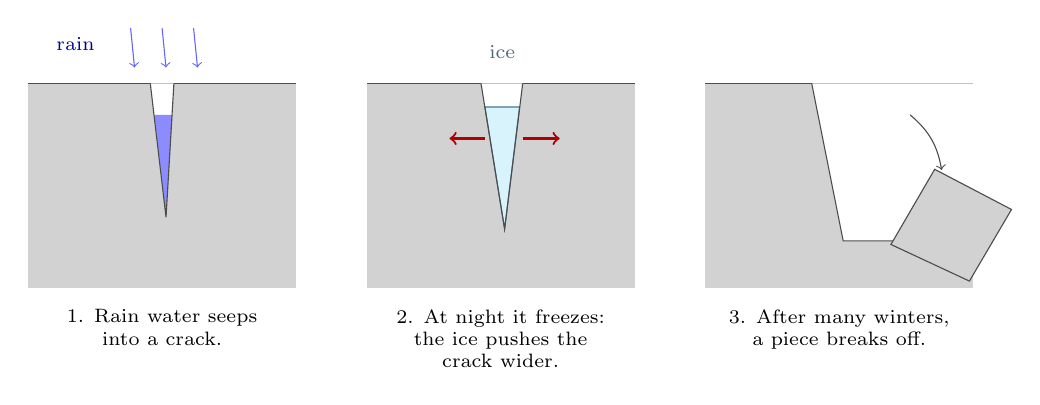
\begin{tikzpicture}[x=1cm, y=1cm, font=\scriptsize]
  \foreach \i/\t in {0/{1. Rain water seeps\\into a crack.},
                     4.3/{2. At night it freezes:\\the ice pushes the\\crack wider.},
                     8.6/{3. After many winters,\\a piece breaks off.}} {
    \begin{scope}[xshift=\i cm]
      \fill[gray!35] (0,0) rectangle (3.4,2.6);
      \draw[gray!60!black] (0,2.6) -- (3.4,2.6);
      \node[align=center, anchor=north] at (1.7,-0.15) {\t};
    \end{scope}
  }
  % panel 1: thin crack with water
  \fill[white] (1.55,2.6) -- (1.75,0.9) -- (1.85,2.6) -- cycle;
  \fill[blue!45] (1.6,2.2) -- (1.75,0.9) -- (1.83,2.2) -- cycle;
  \draw[gray!60!black] (1.55,2.6) -- (1.75,0.9) -- (1.85,2.6);
  \foreach \x in {1.3,1.7,2.1} \draw[blue!60, ->] (\x,3.3) -- (\x+0.05,2.8);
  \node[blue!60!black] at (0.6,3.1) {rain};
  % panel 2: wider crack with ice
  \begin{scope}[xshift=4.3cm]
    \fill[white] (1.45,2.6) -- (1.75,0.75) -- (1.98,2.6) -- cycle;
    \fill[cyan!15] (1.5,2.3) -- (1.75,0.75) -- (1.94,2.3) -- cycle;
    \draw[cyan!50!black] (1.5,2.3) -- (1.75,0.75) -- (1.94,2.3) -- cycle;
    \draw[gray!60!black] (1.45,2.6) -- (1.75,0.75) -- (1.98,2.6);
    \draw[red!70!black, thick, <-] (1.05,1.9) -- (1.5,1.9);
    \draw[red!70!black, thick, ->] (1.98,1.9) -- (2.45,1.9);
    \node[cyan!40!black] at (1.72,3.0) {ice};
  \end{scope}
  % panel 3: broken block
  \begin{scope}[xshift=8.6cm]
    \fill[white] (1.35,2.6) -- (1.75,0.6) -- (3.4,0.6) -- (3.4,2.6) -- cycle;
    \draw[gray!60!black] (1.35,2.6) -- (1.75,0.6) -- (3.4,0.6);
    \fill[gray!35, draw=gray!60!black, rotate around={-25:(2.9,0.3)}]
      (2.3,0.3) -- (2.4,1.4) -- (3.5,1.35) -- (3.4,0.3) -- cycle;
    \draw[gray!60!black, ->] (2.6,2.2) to[bend left=20] (3.0,1.5);
  \end{scope}
\end{tikzpicture}

{\small Frost breaks \omterm{def:g3:stones-pebbles-sand:rock}{rock}. Each night of frost, the ice in a crack pushes a
little; after many winters, the crack is wide enough for a piece to break
away.}
\end{omfigure}

Below a cliff of bare \omterm{def:g3:stones-pebbles-sand:rock}{rock} high in the \omterm{def:g1:landscapes-around-us:landform}{mountains}, the pieces broken off by
the frost slide and tumble down, and pile up in a slope of sharp stones.
They are not rounded: no water has rolled them yet.

\begin{omfigure}
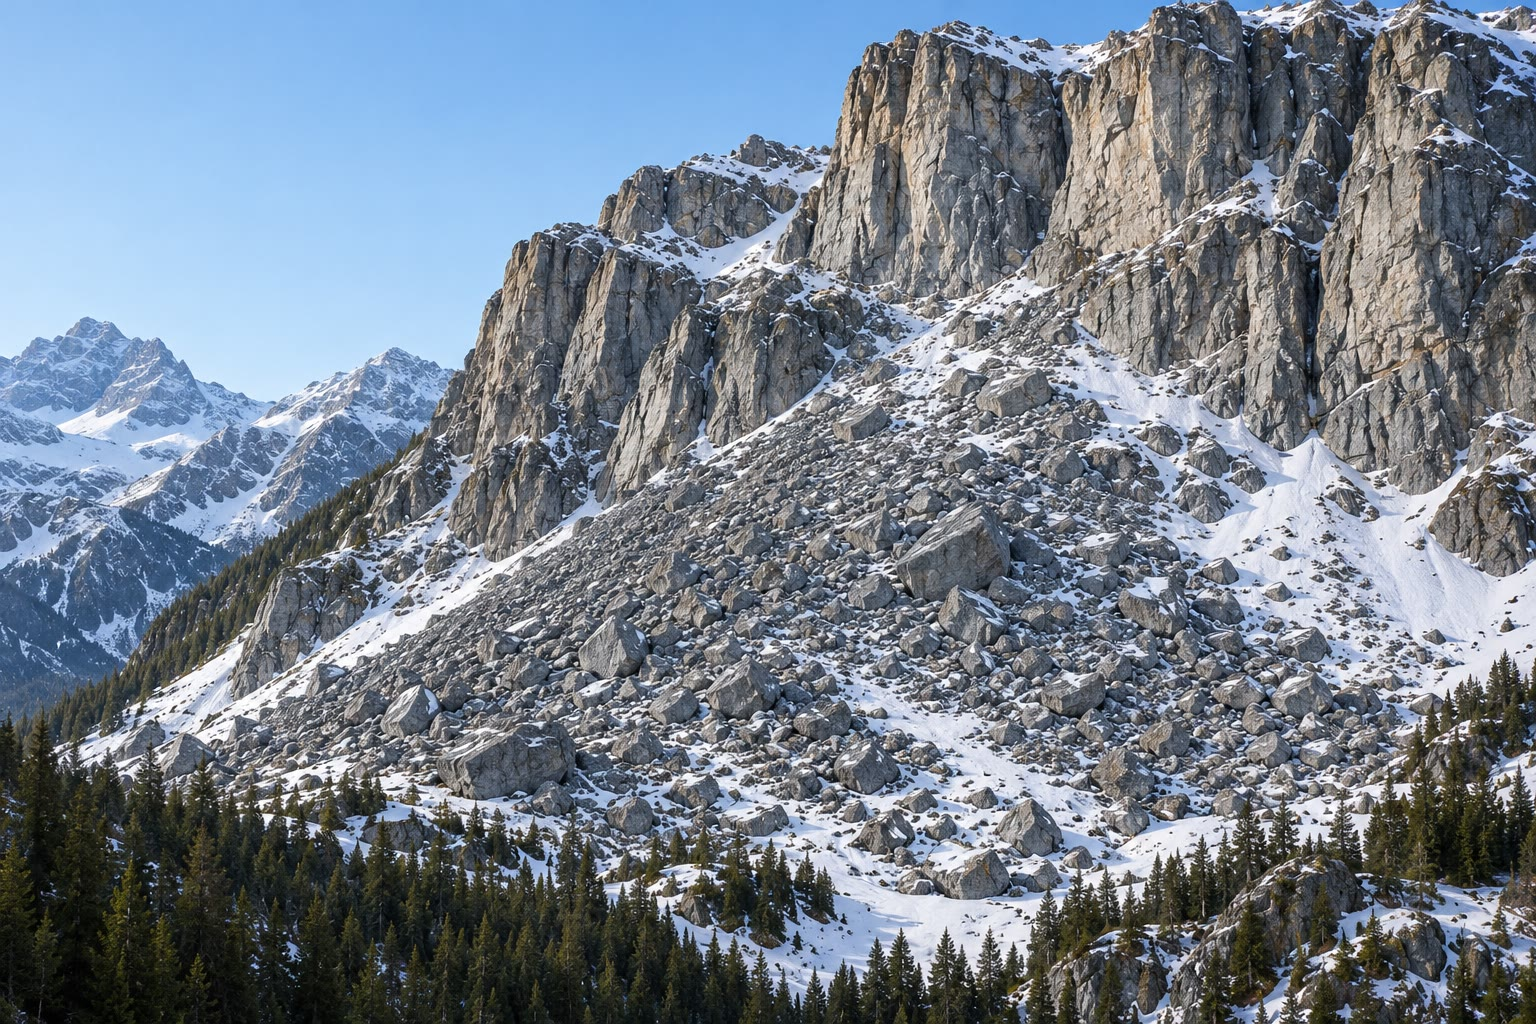
\includegraphics[width=0.5\linewidth]{images/book1/ai/g5-frost-scree.jpg}

{\small Below a \omterm{def:g1:landscapes-around-us:landform}{mountain} cliff, a slope of sharp-edged stones broken off by
frost, seen from across the \omterm{def:g1:landscapes-around-us:landform}{valley}.}
\end{omfigure}

Plants help too. A tree root slips into a crack and, as it grows thicker
year after year, it splits the \omterm{def:g3:stones-pebbles-sand:rock}{rock} like a slow wedge. \omterm{def:g4:clouds-rain-snow:precipitation}{Rain} water itself
slowly softens some \omterm{def:g3:stones-pebbles-sand:rock}{rocks} and turns them into clay and \omterm{def:g3:stones-pebbles-sand:sand}{sand}: that is how
the soil gets its mineral grains.

\section{Water carries the pieces away}

Once the \omterm{def:g3:stones-pebbles-sand:rock}{rock} is broken, the pieces can move. Something must carry them.

\begin{definition}[Erosion]\label{def:g5:water-shapes-the-land:erosion}
\emph{Erosion}\index{erosion} is the wearing-away of the land and the
carrying-away of the pieces of \omterm{def:g3:stones-pebbles-sand:rock}{rock}, by running water above all, but also
by the wind, by ice and by the waves of the \omterm{def:g2:water-on-earth:ocean}{sea}.
\end{definition}

Running water does most of the work. The \omterm{def:g4:clouds-rain-snow:precipitation}{rain} washes soil and grains down
the slopes into the streams; the streams tear more from their own banks,
the way Tom and Lena's stream did after the storm. The faster the water
flows, the more it can carry, and the bigger the pieces it can move: a
calm stream carries only fine \omterm{def:g3:stones-pebbles-sand:sand}{mud}; a stream in \omterm{def:g5:water-shapes-the-land:flood}{flood} rolls \omterm{def:g3:stones-pebbles-sand:pebble}{pebbles} and even
boulders along its bed.

On their way, the stones knock against each other and against the bed.
Their corners break off, and they become rounded \omterm{def:g3:stones-pebbles-sand:pebble}{pebbles}, then smaller and
smaller grains: \omterm{def:g3:stones-pebbles-sand:sand}{sand} and \omterm{def:g3:stones-pebbles-sand:sand}{mud}.

The wind does the same work in dry places, where nothing holds the \omterm{def:g3:stones-pebbles-sand:sand}{sand}:
it blows it into dunes. Ice, in the \omterm{def:g1:landscapes-around-us:landform}{mountains} and near the \omterm{def:g3:continents-and-oceans:poles}{poles}, drags
stones along under its great weight. On the \omterm{def:g1:landscapes-around-us:water}{coast}, waves pound the cliffs
and roll the \omterm{def:g3:stones-pebbles-sand:pebble}{pebbles} of the beach back and forth.

\begin{remark}[How much?]\label{rem:g5:water-shapes-the-land:how-much}
Together, all the \omterm{def:g1:landscapes-around-us:water}{rivers} of the world bring more than 12 billion tonnes of
\omterm{def:g3:stones-pebbles-sand:sand}{mud} and \omterm{def:g3:stones-pebbles-sand:sand}{sand} to the \omterm{def:g2:water-on-earth:ocean}{sea} every year. That is about a billion tonnes every
month.
% ledger: syvitski:modern-flux
\end{remark}

\section{Water lays the pieces down}

A \omterm{def:g1:landscapes-around-us:water}{river} cannot carry its load for ever. Where it slows down, it no longer
has the strength to move its biggest grains, and they settle on the bed.

\begin{definition}[Deposition]\label{def:g5:water-shapes-the-land:deposition}
\emph{Deposition}\index{deposition} is the laying-down of the pieces of \omterm{def:g3:stones-pebbles-sand:rock}{rock}
carried by water, wind or ice, where they slow down and stop.
\end{definition}

The heaviest pieces settle first: \omterm{def:g3:stones-pebbles-sand:pebble}{pebbles} drop where the current slackens a
little, \omterm{def:g3:stones-pebbles-sand:sand}{sand} where it slows more, and the fine \omterm{def:g3:stones-pebbles-sand:sand}{mud} only where the water is
almost still, in a \omterm{def:g1:landscapes-around-us:water}{lake} or in the \omterm{def:g2:water-on-earth:ocean}{sea}. That is why a \omterm{def:g1:landscapes-around-us:water}{river}'s bed is pebbly
in the \omterm{def:g1:landscapes-around-us:landform}{mountains} and sandy or muddy near the \omterm{def:g2:water-on-earth:ocean}{sea}.

\omterm{def:g5:water-shapes-the-land:weathering}{Weathering}, \omterm{def:g5:water-shapes-the-land:erosion}{erosion} and \omterm{def:g5:water-shapes-the-land:deposition}{deposition} are three steps of one long journey:
the \omterm{def:g3:stones-pebbles-sand:rock}{rock} is broken where it stands, its pieces are carried away, and they
are laid down somewhere else. Slowly, water moves the \omterm{def:g1:landscapes-around-us:landform}{mountains}, grain by
grain, down to the \omterm{def:g1:landscapes-around-us:landform}{plains} and into the \omterm{def:g2:water-on-earth:ocean}{sea}.

\begin{method}[Naming what water does]\label{met:g5:water-shapes-the-land:naming}
To name what is happening to \omterm{def:g3:stones-pebbles-sand:rock}{rock} in a picture or a story, ask three
questions:
\begin{enumerate}
  \item Is the \omterm{def:g3:stones-pebbles-sand:rock}{rock} being broken, but the pieces stay where they are?
        That is \emph{\omterm{def:g5:water-shapes-the-land:weathering}{weathering}}.
  \item Are the pieces being worn away and carried off? That is
        \emph{\omterm{def:g5:water-shapes-the-land:erosion}{erosion}}.
  \item Are the pieces settling down and piling up? That is
        \emph{\omterm{def:g5:water-shapes-the-land:deposition}{deposition}}.
\end{enumerate}
\end{method}

\begin{example}[The stream after the storm]\label{ex:g5:water-shapes-the-land:stream}
The brown water of Tom and Lena's stream carries \omterm{def:g3:stones-pebbles-sand:sand}{mud} torn from its banks:
that is \omterm{def:g5:water-shapes-the-land:erosion}{erosion}. A week later, the stream is clear again, and a thin layer
of \omterm{def:g3:stones-pebbles-sand:sand}{mud} covers the bottom of the calm pool at the end of the playground:
that is \omterm{def:g5:water-shapes-the-land:deposition}{deposition}.
\end{example}

\section{A river from its source to its mouth}

Every \omterm{def:g1:landscapes-around-us:water}{river} has a beginning and an end.

\begin{definition}[Source, mouth and tributary]\label{def:g5:water-shapes-the-land:source-mouth}
The \emph{source}\index{source (of a river)} of a \omterm{def:g1:landscapes-around-us:water}{river} is the place where
it begins: a spring, a melting glacier, or a high, wet land where many tiny
streams start. Its \emph{mouth}\index{mouth (of a river)} is the place where
it ends, flowing into the \omterm{def:g2:water-on-earth:ocean}{sea}, a \omterm{def:g1:landscapes-around-us:water}{lake} or a bigger \omterm{def:g1:landscapes-around-us:water}{river}. A
\emph{tributary}\index{tributary} is a smaller \omterm{def:g1:landscapes-around-us:water}{river} that flows into a
bigger one.
\end{definition}

Along its way, a \omterm{def:g1:landscapes-around-us:water}{river} changes. We split its length into three parts, its
upper, middle and lower course.

\begin{omfigure}
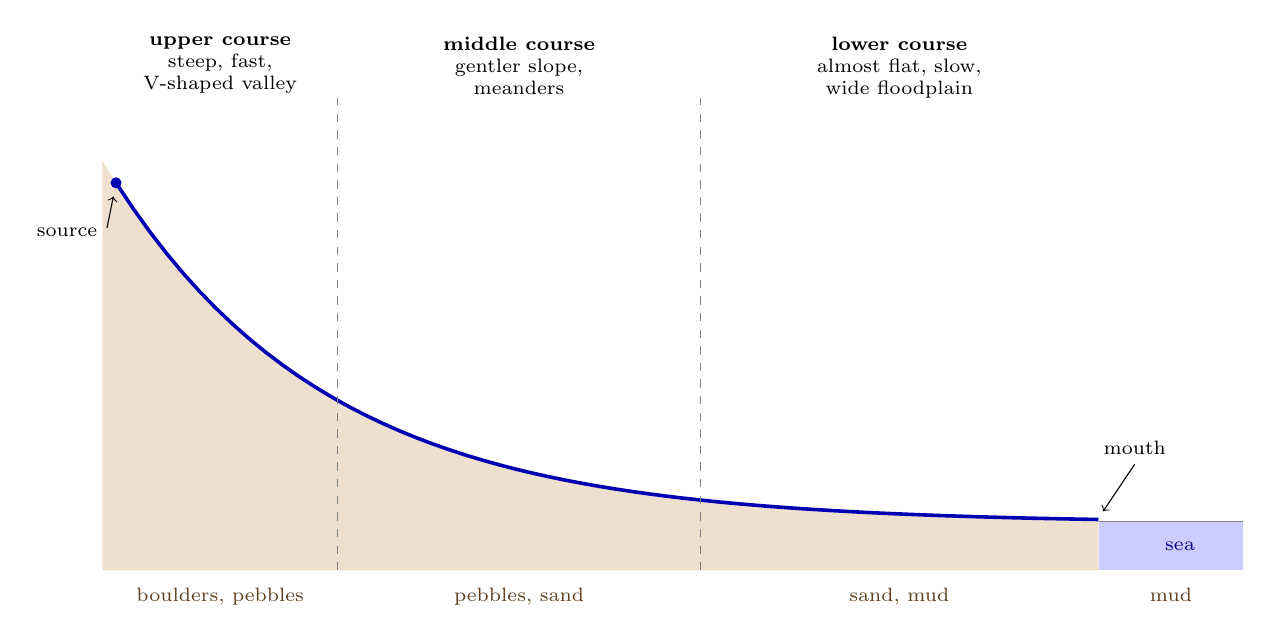
\begin{tikzpicture}[x=1.15cm, y=1cm, font=\scriptsize]
  % ground
  \fill[brown!25] (0,-0.6) -- plot[domain=0:11, samples=60]
    (\x,{4.6*exp(-\x/2.4)}) -- (11,-0.6) -- cycle;
  % sea
  \fill[blue!20] (11,-0.6) rectangle (12.6,0.02);
  \draw[blue!70!black, line width=1.3pt] plot[domain=0.15:11, samples=60]
    (\x,{4.6*exp(-\x/2.4)});
  \draw[gray] (11,0.02) -- (12.6,0.02);
  \node[blue!50!black] at (11.9,-0.3) {sea};
  % course limits
  \foreach \x in {2.6,6.6} \draw[gray, dashed] (\x,-0.6) -- (\x,5.4);
  \node[align=center, anchor=north] at (1.3,6.3) {\textbf{upper course}\\steep, fast,\\V-shaped valley};
  \node[align=center, anchor=north] at (4.6,6.3) {\textbf{middle course}\\gentler slope,\\meanders};
  \node[align=center, anchor=north] at (8.8,6.3) {\textbf{lower course}\\almost flat, slow,\\wide floodplain};
  % source and mouth
  \fill[blue!70!black] (0.15,{4.6*exp(-0.15/2.4)}) circle (2pt);
  \node[anchor=east] at (0.05,3.7) {source};
  \draw[->] (0.05,3.75) -- (0.12,4.15);
  \node[anchor=south] at (11.4,0.75) {mouth};
  \draw[->] (11.4,0.75) -- (11.05,0.15);
  % grain sizes
  \node[anchor=north, align=center, text=brown!50!black] at (1.3,-0.7) {boulders, pebbles};
  \node[anchor=north, align=center, text=brown!50!black] at (4.6,-0.7) {pebbles, sand};
  \node[anchor=north, align=center, text=brown!50!black] at (8.8,-0.7) {sand, mud};
  \node[anchor=north, align=center, text=brown!50!black] at (11.8,-0.7) {mud};
\end{tikzpicture}

{\small The long profile of a \omterm{def:g1:landscapes-around-us:water}{river}, from its \omterm{def:g5:water-shapes-the-land:source-mouth}{source} to its \omterm{def:g5:water-shapes-the-land:source-mouth}{mouth} (the
heights are much stretched). Below: what lies on its bed.}
\end{omfigure}

In its \emph{upper course}, in the \omterm{def:g1:landscapes-around-us:landform}{mountains}, the \omterm{def:g1:landscapes-around-us:water}{river} is young and
steep. Its water rushes down, rolls boulders along its bed and cuts
downwards into the \omterm{def:g3:stones-pebbles-sand:rock}{rock}. It digs a narrow \omterm{def:g1:landscapes-around-us:landform}{valley} with steep sides, shaped
like the letter V.

In its \emph{middle course}, the slope is gentler. The \omterm{def:g1:landscapes-around-us:water}{river} swings from
side to side in great loops.

\begin{definition}[Meander]\label{def:g5:water-shapes-the-land:meander}
A \emph{meander}\index{meander} is a loop of a \omterm{def:g1:landscapes-around-us:water}{river} that winds across a
flat \omterm{def:g1:landscapes-around-us:landform}{valley} floor.
\end{definition}

A \omterm{def:g5:water-shapes-the-land:meander}{meander} does not stay still: it moves. On the outside of each bend, the
water flows fast and deep: it eats into the bank, which becomes a small
cliff. On the inside of the bend, the water flows slowly: it drops \omterm{def:g3:stones-pebbles-sand:sand}{sand} and
\omterm{def:g3:stones-pebbles-sand:pebble}{gravel}, which build a gentle beach. Year after year, the outer bank is worn
back and the inner beach grows, and the loop swings wider and wider.

\begin{omfigure}
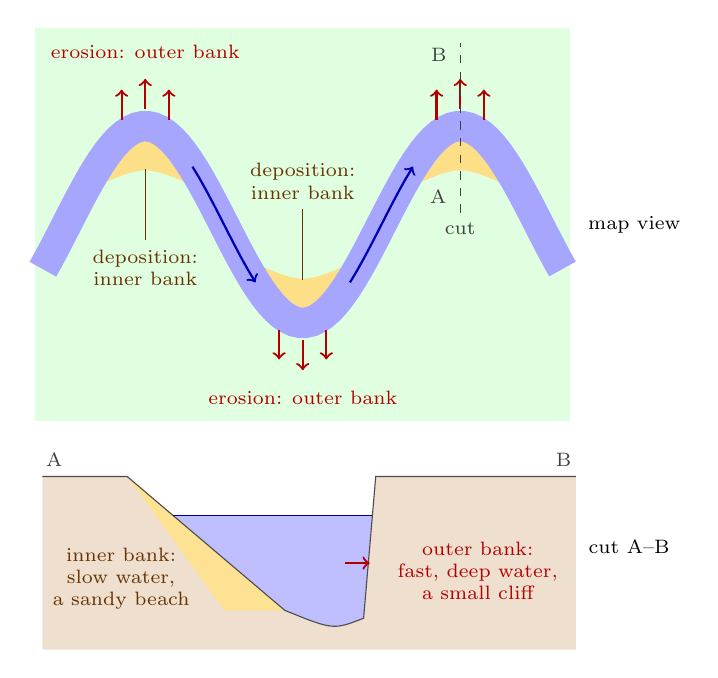
\begin{tikzpicture}[x=1cm, y=1cm, font=\scriptsize]
  % ---- map view ----
  \fill[green!12] (-0.4,-2.5) rectangle (6.4,2.5);
  % sand on the inner banks (drawn first, the river covers its edge)
  \foreach \c/\s in {1/1, 3/-1, 5/1}
    \fill[yellow!50!orange!45] (\c-0.6,\s*0.5) .. controls (\c,\s*1.5) ..
      (\c+0.6,\s*0.5) .. controls (\c,\s*0.75) .. cycle;
  % the river
  \draw[blue!35, line width=11pt] plot[domain=-0.3:6.3, samples=90]
    (\x,{1.25*sin(\x*90)});
  \draw[blue!70!black, ->, thick] plot[domain=1.6:2.4, samples=10]
    (\x,{1.25*sin(\x*90)});
  \draw[blue!70!black, ->, thick] plot[domain=3.6:4.4, samples=10]
    (\x,{1.25*sin(\x*90)});
  % erosion on the outer banks
  \foreach \c/\s in {1/1, 3/-1, 5/1}
    \foreach \d in {-0.3,0,0.3}
      \draw[red!70!black, thick, ->] (\c+\d,{\s*(1.25*cos(\d*90)+0.22)})
        -- (\c+\d,{\s*(1.25*cos(\d*90)+0.6)});
  \node[red!70!black] at (1,2.2) {erosion: outer bank};
  \node[red!70!black] at (3,-2.2) {erosion: outer bank};
  \node[orange!40!black, align=center] (d1) at (1,-0.55) {deposition:\\inner bank};
  \node[orange!40!black, align=center] (d2) at (3,0.55) {deposition:\\inner bank};
  \draw[orange!40!black] (d1.north) -- (1,0.7);
  \draw[orange!40!black] (d2.south) -- (3,-0.7);
  \draw[gray!50!black, dashed] (5,0.15) -- (5,2.3);
  \node[gray!50!black, anchor=north] at (5,0.15) {cut};
  \node[gray!50!black, anchor=east] at (4.95,0.35) {A};
  \node[gray!50!black, anchor=east] at (4.95,2.15) {B};
  \node[anchor=west] at (6.5,0) {map view};
  % ---- cut ----
  \begin{scope}[yshift=-4.1cm, xscale=0.77]
    \fill[brown!25] (-0.4,-1.3) -- (-0.4,0.9) -- (1,0.9) -- (3.6,-0.8)
      .. controls (4.4,-1.05) .. (4.9,-0.9) -- (5.1,0.9) -- (8.4,0.9)
      -- (8.4,-1.3) -- cycle;
    \fill[blue!25] (1.75,0.4) -- (3.6,-0.8) .. controls (4.4,-1.05) .. (4.9,-0.9)
      -- (5.04,0.4) -- cycle;
    \fill[yellow!50!orange!40] (1,0.9) -- (3.6,-0.8) -- (2.6,-0.8) -- cycle;
    \draw[gray!60!black] (-0.4,0.9) -- (1,0.9) -- (3.6,-0.8)
      .. controls (4.4,-1.05) .. (4.9,-0.9) -- (5.1,0.9) -- (8.4,0.9);
    \draw[blue!60!black] (1.75,0.4) -- (5.04,0.4);
    \node[orange!40!black, align=center] at (0.9,-0.4) {inner bank:\\slow water,\\a sandy beach};
    \node[red!70!black, align=center, anchor=west] at (5.3,-0.3) {outer bank:\\fast, deep water,\\a small cliff};
    \draw[red!70!black, thick, ->] (4.6,-0.2) -- (5.0,-0.2);
    \node[gray!50!black, anchor=south] at (-0.2,0.9) {A};
    \node[gray!50!black, anchor=south] at (8.2,0.9) {B};
    \node[anchor=west] at (8.45,0) {cut A--B};
  \end{scope}
\end{tikzpicture}

{\small A \omterm{def:g5:water-shapes-the-land:meander}{meander} seen from above, and cut across along the dashed line A--B.
The water wears away the outer bank of each bend and drops \omterm{def:g3:stones-pebbles-sand:sand}{sand} on the
inner bank: the loop slowly moves.}
\end{omfigure}

Sometimes two loops grow so close that, during a \omterm{def:g5:water-shapes-the-land:flood}{flood}, the \omterm{def:g1:landscapes-around-us:water}{river} breaks
through the narrow neck of land between them and takes the short cut. The
old loop is left behind as a curved \omterm{def:g1:landscapes-around-us:water}{lake}.

\begin{omfigure}
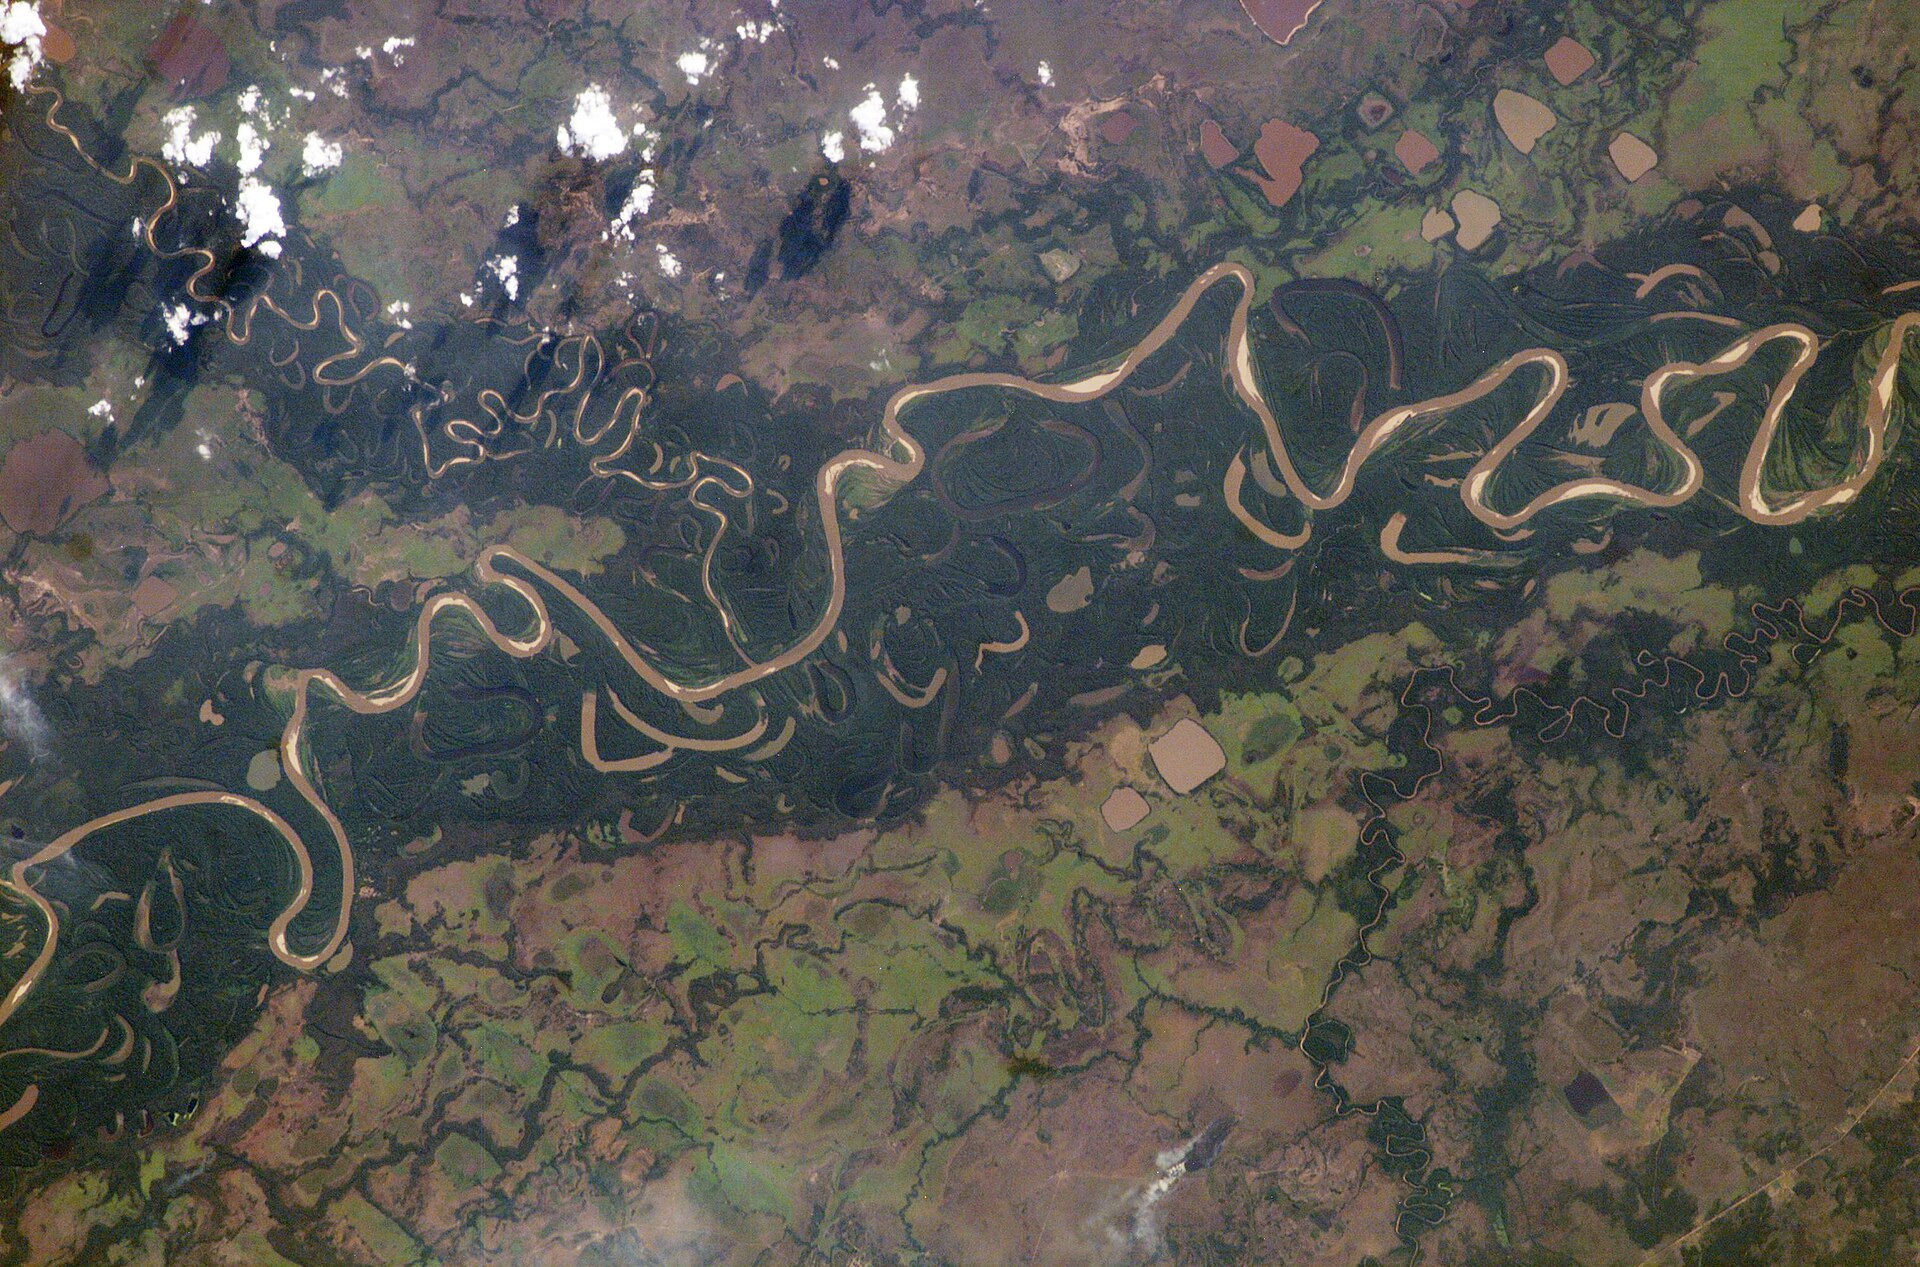
\includegraphics[width=0.52\linewidth]{images/book1/g5-mamore-meanders.jpg}

{\small The Mamoré \omterm{def:g1:landscapes-around-us:water}{River}, in the lowlands of Bolivia in South America, seen
from the International Space Station. The brown \omterm{def:g1:landscapes-around-us:water}{river} winds in \omterm{def:g5:water-shapes-the-land:meander}{meanders}
through the forest. Photograph: NASA (public domain).}\label{fig:g5:water-shapes-the-land:mamore}
% ledger: nasa:mamore-meanders
\end{omfigure}

In its \emph{lower course}, the land is almost flat. The \omterm{def:g1:landscapes-around-us:water}{river} flows slowly
across a wide, flat \omterm{def:g1:landscapes-around-us:landform}{valley} floor, made of the \omterm{def:g3:stones-pebbles-sand:sand}{mud} and \omterm{def:g3:stones-pebbles-sand:sand}{sand} it has laid down
itself over a very long time.

\begin{omfigure}
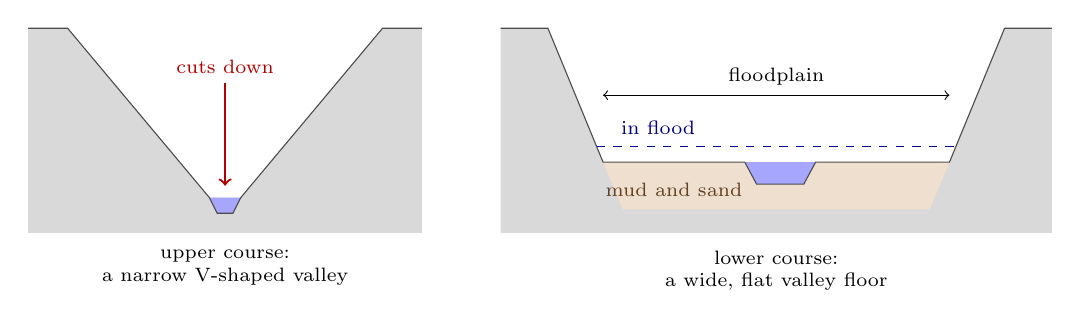
\begin{tikzpicture}[x=1cm, y=1cm, font=\scriptsize]
  % V-shaped valley
  \fill[gray!30] (0,0) -- (0,2.6) -- (0.5,2.6) -- (2.3,0.45) -- (2.7,0.45)
    -- (4.5,2.6) -- (5,2.6) -- (5,0) -- cycle;
  \fill[blue!35] (2.3,0.45) -- (2.4,0.25) -- (2.6,0.25) -- (2.7,0.45) -- cycle;
  \draw[gray!60!black] (0,2.6) -- (0.5,2.6) -- (2.3,0.45) -- (2.4,0.25)
    -- (2.6,0.25) -- (2.7,0.45) -- (4.5,2.6) -- (5,2.6);
  \draw[red!70!black, thick, ->] (2.5,1.9) -- (2.5,0.6);
  \node[red!70!black, anchor=south] at (2.5,1.9) {cuts down};
  \node[align=center, anchor=north] at (2.5,-0.1) {upper course:\\a narrow V-shaped valley};
  % floodplain
  \begin{scope}[xshift=6cm]
    \fill[gray!30] (0,0) -- (0,2.6) -- (0.6,2.6) -- (1.3,0.9) -- (5.7,0.9)
      -- (6.4,2.6) -- (7,2.6) -- (7,0) -- cycle;
    \fill[brown!25] (1.3,0.9) -- (1.55,0.3) -- (5.45,0.3) -- (5.7,0.9) -- cycle;
    \fill[blue!35] (3.1,0.9) -- (3.25,0.62) -- (3.85,0.62) -- (4,0.9) -- cycle;
    \draw[gray!60!black] (0,2.6) -- (0.6,2.6) -- (1.3,0.9) -- (3.1,0.9)
      -- (3.25,0.62) -- (3.85,0.62) -- (4,0.9) -- (5.7,0.9) -- (6.4,2.6) -- (7,2.6);
    \draw[blue!60!black, dashed] (1.22,1.1) -- (5.78,1.1);
    \node[blue!50!black, anchor=south] at (2.0,1.12) {in flood};
    \node[brown!50!black] at (2.2,0.55) {mud and sand};
    \draw[<->] (1.3,1.75) -- (5.7,1.75);
    \node[anchor=south] at (3.5,1.75) {floodplain};
    \node[align=center, anchor=north] at (3.5,-0.1) {lower course:\\a wide, flat valley floor};
  \end{scope}
\end{tikzpicture}

{\small The \omterm{def:g1:landscapes-around-us:landform}{valley} cut across, in the \omterm{def:g1:landscapes-around-us:landform}{mountains} and near the \omterm{def:g2:water-on-earth:ocean}{sea} (not to the
same scale). In \omterm{def:g5:water-shapes-the-land:flood}{flood}, the \omterm{def:g1:landscapes-around-us:water}{river} spreads over its whole \omterm{def:g5:water-shapes-the-land:flood}{floodplain}.}
\end{omfigure}

At last the \omterm{def:g1:landscapes-around-us:water}{river} reaches its \omterm{def:g5:water-shapes-the-land:source-mouth}{mouth}. There the water slows down almost
completely, and the \omterm{def:g1:landscapes-around-us:water}{river} drops the last of its load. Where the waves and
the tides of the \omterm{def:g2:water-on-earth:ocean}{sea} are too weak to carry all of it away, the \omterm{def:g3:stones-pebbles-sand:sand}{mud} and \omterm{def:g3:stones-pebbles-sand:sand}{sand}
pile up, and new land grows out into the \omterm{def:g2:water-on-earth:ocean}{sea}.

\begin{definition}[Delta]\label{def:g5:water-shapes-the-land:delta}
A \emph{delta}\index{delta} is new, flat land built by a \omterm{def:g1:landscapes-around-us:water}{river} at its \omterm{def:g5:water-shapes-the-land:source-mouth}{mouth}
from the \omterm{def:g3:stones-pebbles-sand:sand}{mud} and \omterm{def:g3:stones-pebbles-sand:sand}{sand} it lays down. The \omterm{def:g1:landscapes-around-us:water}{river} splits into several branches
that spread across it, often in the shape of a fan.
\end{definition}

The name comes from the Greek letter $\Delta$ (\omterm{def:g5:water-shapes-the-land:delta}{delta}), a triangle,
because the \omterm{def:g5:water-shapes-the-land:delta}{delta} of the Nile, in Egypt, has that shape.

Some \omterm{def:g1:landscapes-around-us:water}{rivers} end without a \omterm{def:g5:water-shapes-the-land:delta}{delta}. Where strong waves and tides sweep the
\omterm{def:g3:stones-pebbles-sand:sand}{mud} away, the \omterm{def:g1:landscapes-around-us:water}{river} ends in a wide, funnel-shaped \omterm{def:g5:water-shapes-the-land:source-mouth}{mouth} where the \omterm{def:g2:water-on-earth:ocean}{sea} comes
in and out with the tides: an \emph{estuary}.

\begin{omfigure}
\begin{minipage}[b]{0.55\linewidth}\centering
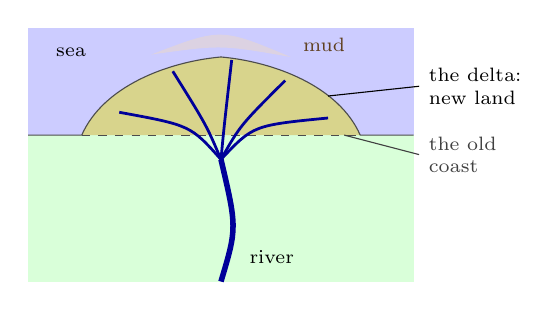
\begin{tikzpicture}[x=0.68cm, y=0.62cm, font=\scriptsize]
  \fill[blue!20] (-3.6,1.4) rectangle (3.6,3.6);
  \fill[green!15] (-3.6,-1.6) rectangle (3.6,1.4);
  % delta
  \fill[olive!35] (-2.6,1.4) .. controls (-2.2,2.4) and (-1,2.9)
    .. (0,3.0) .. controls (1,2.9) and (2.2,2.4) .. (2.6,1.4) -- cycle;
  \draw[gray!60!black] (-3.6,1.4) -- (-2.6,1.4) .. controls (-2.2,2.4) and
    (-1,2.9) .. (0,3.0) .. controls (1,2.9) and (2.2,2.4) .. (2.6,1.4) -- (3.6,1.4);
  \draw[gray!60!black, dashed] (-2.6,1.4) -- (2.6,1.4);
  % river and branches
  \draw[blue!60!black, line width=2pt] (0,-1.6) .. controls (0.3,-0.5) .. (0,0.9);
  \foreach \e in {-1.9,-0.9,0.2,1.2,2.0}
    \draw[blue!60!black, line width=1pt] (0,0.9) .. controls (\e*0.3,1.6) ..
      (\e,{2.95-0.3*\e*\e});
  % mud plume
  \fill[brown!30, opacity=0.5] (-1.3,3.05) .. controls (0,3.6) .. (1.3,3.0)
    .. controls (0,3.25) .. cycle;
  \node[align=center] at (-2.8,3.1) {sea};
  \node[anchor=west, brown!50!black] at (1.35,3.25) {mud};
  \node[anchor=west, align=left] at (3.7,2.4) {the delta:\\new land};
  \draw (3.7,2.4) -- (2.0,2.2);
  \node[anchor=west, align=left, gray!50!black] at (3.7,1.0) {the old\\coast};
  \draw[gray!50!black] (3.7,1.0) -- (2.3,1.4);
  \node[anchor=west] at (0.35,-1.1) {river};
\end{tikzpicture}
\end{minipage}\hfill
\begin{minipage}[b]{0.3\linewidth}\centering
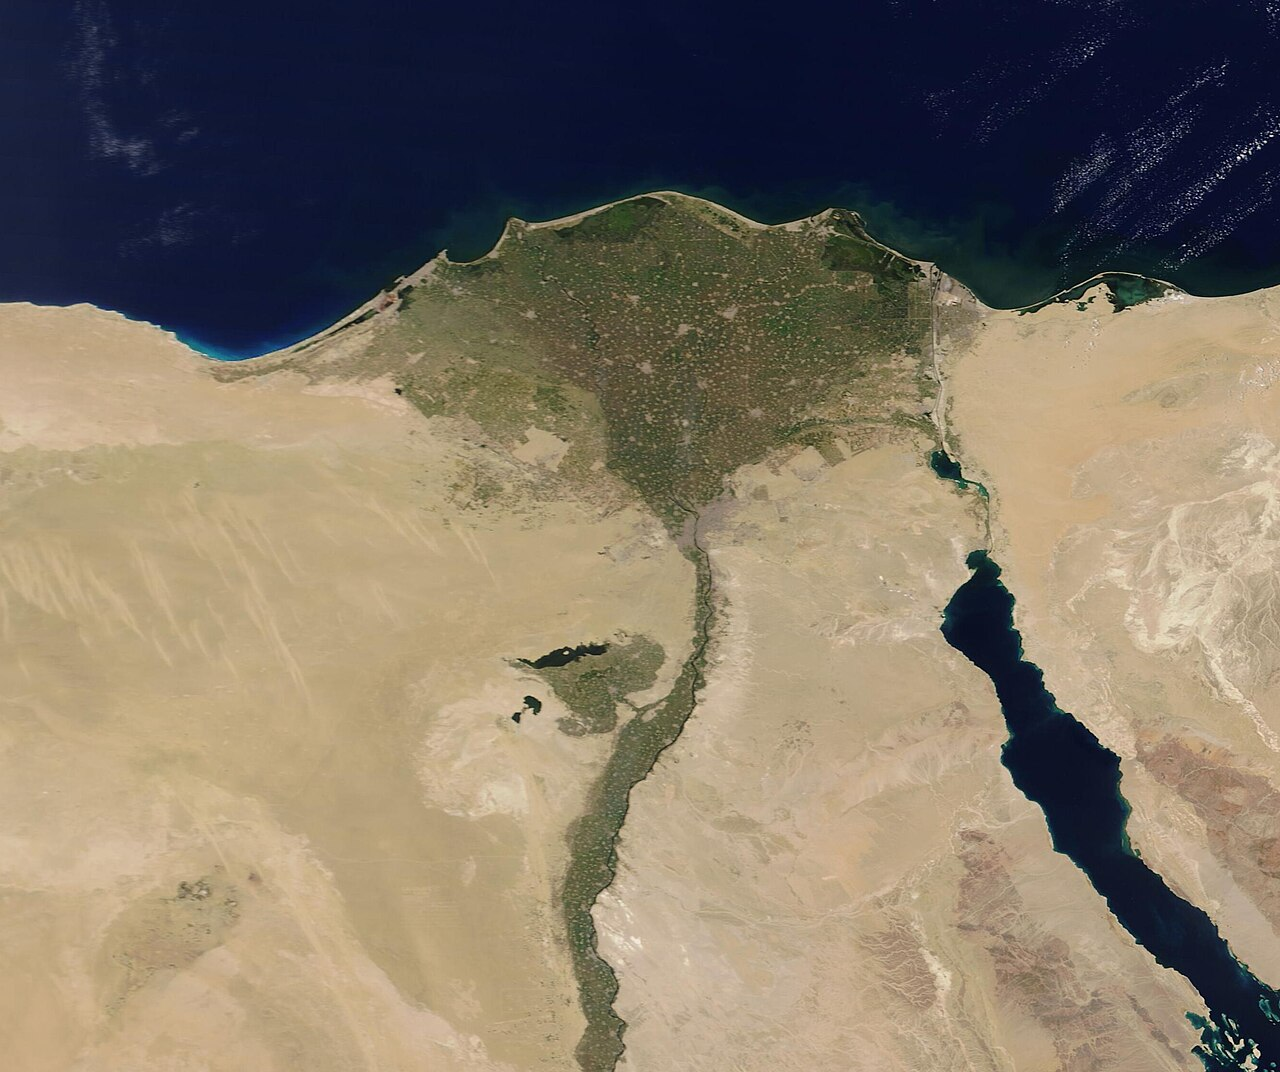
\includegraphics[width=\linewidth]{images/book1/g5-nile-delta-modis.jpg}
\end{minipage}

{\small Left: a \omterm{def:g5:water-shapes-the-land:delta}{delta} seen from above; the \omterm{def:g3:stones-pebbles-sand:sand}{mud} and \omterm{def:g3:stones-pebbles-sand:sand}{sand} laid down by the
branches build new land beyond the old \omterm{def:g1:landscapes-around-us:water}{coast}. Right: the Nile \omterm{def:g5:water-shapes-the-land:delta}{delta}, in
Egypt, from a satellite (\omterm{def:g2:water-on-earth:ocean}{sea} at the top): a green fan of fields on the
\omterm{def:g1:landscapes-around-us:water}{river}'s \omterm{def:g3:stones-pebbles-sand:sand}{mud}, in the middle of the desert. Photograph: NASA (public
domain).}
% ledger: nasa:nile-delta-modis
\end{omfigure}

\section{Floods}

After long days of \omterm{def:g4:clouds-rain-snow:precipitation}{rain}, or when the \omterm{def:g4:clouds-rain-snow:precipitation}{snow} melts fast in spring, a \omterm{def:g1:landscapes-around-us:water}{river}
receives more water than its channel can hold.

\begin{definition}[Flood and floodplain]\label{def:g5:water-shapes-the-land:flood}
A \emph{flood}\index{flood} happens when water covers land that is usually
dry. A \omterm{def:g1:landscapes-around-us:water}{river} floods when it rises above its banks and spreads over the
flat land on either side of it. That flat land, which the \omterm{def:g1:landscapes-around-us:water}{river} covers from
time to time, is its \emph{floodplain}\index{floodplain}.
\end{definition}

\begin{omfigure}
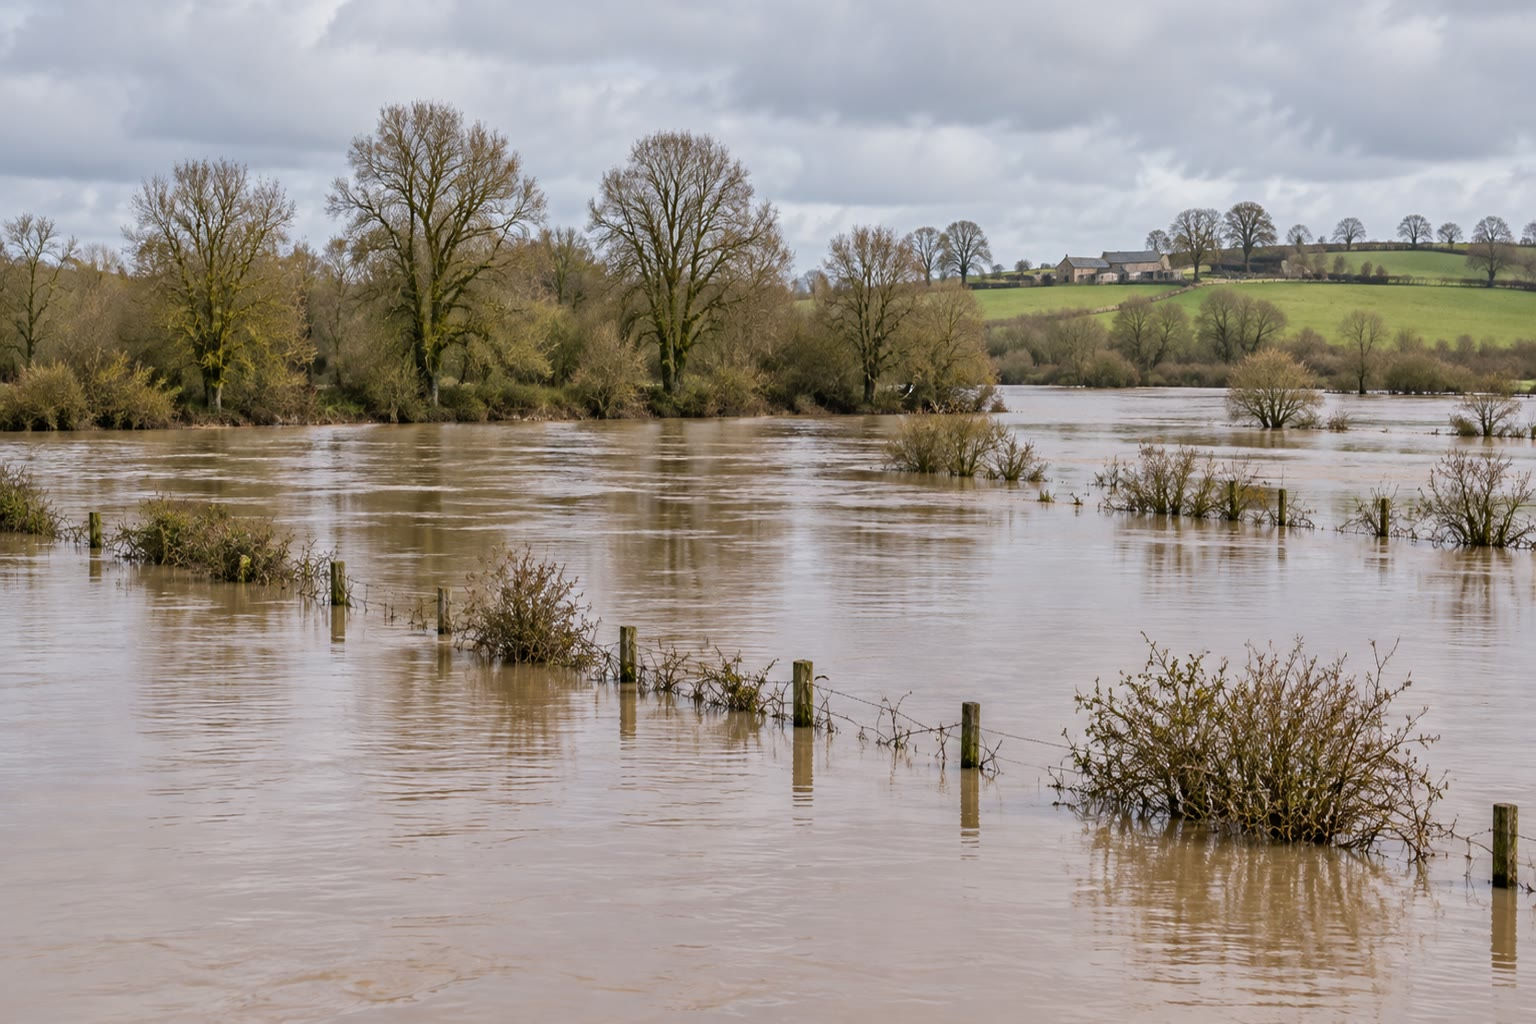
\includegraphics[width=0.5\linewidth]{images/book1/ai/g5-flooded-meadow.jpg}

{\small A meadow under \omterm{def:g5:water-shapes-the-land:flood}{flood} water after days of \omterm{def:g4:clouds-rain-snow:precipitation}{rain}. The line of trees
marks the \omterm{def:g1:landscapes-around-us:water}{river}'s usual bank; the farm stands on higher ground.}
\end{omfigure}

A \omterm{def:g1:landscapes-around-us:water}{river} that \omterm{def:g5:water-shapes-the-land:flood}{floods} is not doing anything strange: it is doing what \omterm{def:g1:landscapes-around-us:water}{rivers}
have always done. The \omterm{def:g5:water-shapes-the-land:flood}{floodplain} is its territory. In fact the \omterm{def:g1:landscapes-around-us:water}{river} built
it: each \omterm{def:g5:water-shapes-the-land:flood}{flood} leaves behind a thin layer of \omterm{def:g3:stones-pebbles-sand:sand}{mud} on the fields, which is
why \omterm{def:g5:water-shapes-the-land:flood}{floodplains} have such rich soil. Long ago, farmers in
Egypt waited for the yearly \omterm{def:g5:water-shapes-the-land:flood}{flood} of the Nile, which watered their fields
and brought them new \omterm{def:g3:stones-pebbles-sand:sand}{mud}.

But a \omterm{def:g5:water-shapes-the-land:flood}{flood} is dangerous for people who live on the \omterm{def:g5:water-shapes-the-land:flood}{floodplain}. Houses
built on it can be filled with water, and fast \omterm{def:g5:water-shapes-the-land:flood}{flood} water can sweep away
cars and people. A wise town builds on higher ground and leaves the
\omterm{def:g5:water-shapes-the-land:flood}{floodplain} to fields, meadows and parks. In \cref{ch:g5:natural-hazards}
we will see how people prepare for \omterm{def:g5:water-shapes-the-land:flood}{floods} and stay safe.

\begin{safety}
Never walk, cycle or play in \omterm{def:g5:water-shapes-the-land:flood}{flood} water, and never go near a \omterm{def:g1:landscapes-around-us:water}{river} in
\omterm{def:g5:water-shapes-the-land:flood}{flood}: the water is stronger and deeper than it looks, and it can hide
holes and open drains. Keep away until the grown-ups in charge say it is
safe.
\end{safety}

\section{Exercises}

\begin{exercise}[$\star$]\label{exo:g5:water-shapes-the-land:1}
Name the process: \omterm{def:g5:water-shapes-the-land:weathering}{weathering}, \omterm{def:g5:water-shapes-the-land:erosion}{erosion} or \omterm{def:g5:water-shapes-the-land:deposition}{deposition}?
\begin{enumerate}
  \item[(a)] Ice in a crack splits a \omterm{def:g3:stones-pebbles-sand:rock}{rock} on a \omterm{def:g1:landscapes-around-us:landform}{mountain}.
  \item[(b)] A \omterm{def:g1:landscapes-around-us:water}{river} in \omterm{def:g5:water-shapes-the-land:flood}{flood} carries \omterm{def:g3:stones-pebbles-sand:sand}{sand} away from its banks.
  \item[(c)] A layer of \omterm{def:g3:stones-pebbles-sand:sand}{mud} settles at the bottom of a calm \omterm{def:g1:landscapes-around-us:water}{lake}.
  \item[(d)] A tree root splits a stone wall.
\end{enumerate}
\end{exercise}

\begin{exercise}[$\star$]\label{exo:g5:water-shapes-the-land:2}
What is the source of a \omterm{def:g1:landscapes-around-us:water}{river}? What is its \omterm{def:g5:water-shapes-the-land:source-mouth}{mouth}? What is a \omterm{def:g5:water-shapes-the-land:source-mouth}{tributary}?
\end{exercise}

\begin{exercise}[$\star$]\label{exo:g5:water-shapes-the-land:3}
Put these parts of a \omterm{def:g1:landscapes-around-us:water}{river} in order, from the \omterm{def:g5:water-shapes-the-land:source-mouth}{source} to the \omterm{def:g2:water-on-earth:ocean}{sea}: the
\omterm{def:g5:water-shapes-the-land:meander}{meanders}; the \omterm{def:g5:water-shapes-the-land:delta}{delta}; the narrow V-shaped \omterm{def:g1:landscapes-around-us:landform}{valley}; the \omterm{def:g5:water-shapes-the-land:source-mouth}{source}.
\end{exercise}

\begin{exercise}[$\star$]\label{exo:g5:water-shapes-the-land:4}
True or false? Explain.
\begin{enumerate}
  \item[(a)] Hard \omterm{def:g3:stones-pebbles-sand:rock}{rock} never changes.
  \item[(b)] A fast \omterm{def:g1:landscapes-around-us:water}{river} can carry bigger stones than a slow \omterm{def:g1:landscapes-around-us:water}{river}.
  \item[(c)] The finest \omterm{def:g3:stones-pebbles-sand:sand}{mud} settles first, near the \omterm{def:g5:water-shapes-the-land:source-mouth}{source}.
\end{enumerate}
\end{exercise}

\begin{exercise}[$\star$]\label{exo:g5:water-shapes-the-land:5}
Here is a bend of a \omterm{def:g1:landscapes-around-us:water}{river} seen from above.

\begin{center}
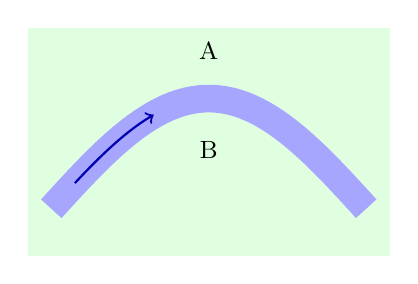
\begin{tikzpicture}[x=1cm, y=1cm, font=\small]
  \fill[green!12] (-0.3,-0.6) rectangle (4.3,2.3);
  \draw[blue!35, line width=10pt] plot[domain=0:4, samples=50]
    (\x,{1.4*sin(\x*45)});
  \draw[blue!70!black, ->, thick] plot[domain=0.3:1.3, samples=20]
    (\x,{1.4*sin(\x*45)});
  \node at (2,2.0) {A};
  \node at (2,0.75) {B};
\end{tikzpicture}
\end{center}
On which bank, A or B, does the \omterm{def:g1:landscapes-around-us:water}{river} wear the land away? On which bank
does it drop \omterm{def:g3:stones-pebbles-sand:sand}{sand}?
\end{exercise}

\begin{exercise}[$\star$]\label{exo:g5:water-shapes-the-land:6}
In the \omterm{def:g1:landscapes-around-us:landform}{mountains}, the bed of a \omterm{def:g1:landscapes-around-us:water}{river} is covered with large stones. Near the
\omterm{def:g2:water-on-earth:ocean}{sea}, it is covered with \omterm{def:g3:stones-pebbles-sand:sand}{sand} and \omterm{def:g3:stones-pebbles-sand:sand}{mud}. Why?
\end{exercise}

\begin{exercise}[$\star\star$]\label{exo:g5:water-shapes-the-land:7}
A \omterm{def:g1:landscapes-around-us:water}{river} is 600 kilometres long. Its upper course is the first
$\frac{1}{6}$ of its length, and its middle course the next
$\frac{1}{2}$.
\begin{enumerate}
  \item[(a)] How long is the upper course? the middle course?
  \item[(b)] How long is the lower course? What fraction of the \omterm{def:g1:landscapes-around-us:water}{river} is
        it?
\end{enumerate}
\end{exercise}

\begin{exercise}[$\star\star$]\label{exo:g5:water-shapes-the-land:8}
Look again at the photograph of the Mamoré \omterm{def:g1:landscapes-around-us:water}{River} seen from the space
station, on page~\pageref{fig:g5:water-shapes-the-land:mamore}. What are the pale patches on the inside of the
bends? What are the dark curved \omterm{def:g1:landscapes-around-us:water}{lakes} beside the \omterm{def:g1:landscapes-around-us:water}{river}? How were they made?
\end{exercise}

\begin{exercise}[$\star\star$]\label{exo:g5:water-shapes-the-land:9}
A town wants to build a new school in the flat green meadows beside its
\omterm{def:g1:landscapes-around-us:water}{river}, because the land there is flat and cheap. What would you tell the
town council? Use the words \emph{\omterm{def:g5:water-shapes-the-land:flood}{flood}} and \emph{\omterm{def:g5:water-shapes-the-land:flood}{floodplain}}.
\end{exercise}

\begin{exercise}[$\star\star$]\label{exo:g5:water-shapes-the-land:10}
The \omterm{def:g1:landscapes-around-us:water}{rivers} of the world bring about 12 billion tonnes of \omterm{def:g3:stones-pebbles-sand:sand}{mud} and \omterm{def:g3:stones-pebbles-sand:sand}{sand} to
the \omterm{def:g2:water-on-earth:ocean}{sea} every year.
\begin{enumerate}
  \item[(a)] How many tonnes is that every month, on average?
  \item[(b)] A big lorry carries 10 tonnes. How many lorry-loads would it
        take to carry one month's \omterm{def:g3:stones-pebbles-sand:sand}{mud} and \omterm{def:g3:stones-pebbles-sand:sand}{sand}?
\end{enumerate}
\end{exercise}

\begin{exercise}[$\star\star\star$]\label{exo:g5:water-shapes-the-land:11}
Tell the story of a grain of \omterm{def:g3:stones-pebbles-sand:sand}{sand}. It starts as part of a \omterm{def:g3:stones-pebbles-sand:rock}{rock} high on a
\omterm{def:g1:landscapes-around-us:landform}{mountain}, and it ends, many years later, in a \omterm{def:g5:water-shapes-the-land:delta}{delta}. Use the words
\emph{\omterm{def:g5:water-shapes-the-land:weathering}{weathering}}, \emph{\omterm{def:g5:water-shapes-the-land:erosion}{erosion}} and \emph{\omterm{def:g5:water-shapes-the-land:deposition}{deposition}}, and say what
happens to the grain in the upper, middle and lower course of the \omterm{def:g1:landscapes-around-us:water}{river}.
\end{exercise}
